\documentclass[11pt,a4paper]{article}
\usepackage[T1]{fontenc}
\usepackage{lmodern,microtype,amsmath,amssymb,amsthm,booktabs}
\usepackage[margin=27mm]{geometry}
\usepackage{tikz,hyperref,float}
\usetikzlibrary{arrows.meta,positioning,calc}
\hypersetup{colorlinks=true,urlcolor=blue,linkcolor=black,citecolor=black}
\emergencystretch=3em
\newtheorem{theorem}{Theorem}
\newtheorem{lemma}[theorem]{Lemma}
\newtheorem{proposition}[theorem]{Proposition}
\newcommand{\PalomarEntry}{\href{https://palomar-registry.org/entry.html?id=PALOMAR-2026-10-27-000023\&version=1}{\texttt{PALOMAR-2026-10-27-000023, v1}}}
\newcommand{\Gcoords}{%
\coordinate (v0) at (-2.8,0);\coordinate (v3) at (-.8,0);
\coordinate (v5) at (-1.8,1.2);\coordinate (v6) at (-1.8,-1.2);
\coordinate (v1) at (2.6,0);\coordinate (v4) at (4.6,0);
\coordinate (v7) at (3.6,1.2);\coordinate (v8) at (3.6,-1.2);
\coordinate (v2) at (.9,-2.5);}
\newcommand{\Gedges}{\foreach \a/\b in {0/3,0/5,0/6,1/4,1/7,1/8,2/6,2/8,3/5,3/6,4/7,4/8,5/7,6/8}{\draw[line width=.7pt] (v\a)--(v\b);}}
\newcommand{\Gvertices}{\foreach \i in {0,1,2,3,4,5,6,7,8}{\node[draw,fill=white,circle,inner sep=0pt,minimum size=7mm,font=\small\bfseries] at (v\i) {\i};}}
\title{Counterexamples to the Pointwise and Critical Almost Stacked Hypotheses}
\author{John Fairfax-Ball\\{\small Independent researcher, United Kingdom}}
\date{}
\begin{document}
\maketitle
\begin{abstract}
The Almost Stacked Hypothesis of Csern\'ak and Soukup has a printed
pointwise formulation and a natural critical (largest-losing-layer)
formulation. The former fails already for stacking on a four-vertex path
and clearing on a five-vertex bull graph. More substantially, a connected
non-bipartite nine-vertex graph refutes both clauses of the critical form.
Its stacking and clearing thresholds are $15$, but its only mass-$14$
losers are two non-almost-stacked automorphic configurations.
The decisive finite result has been certified using Lean and independently
reproducible reachability computations.
\end{abstract}

\noindent\textbf{Keywords:} graph pebbling; stacking number; clearing number;
counterexample; formal verification.

\noindent\textbf{2020 Mathematics Subject Classification:}
05C57 (primary); 05C85 (secondary).

\section{Introduction}
Csern\'ak and Soukup introduced the stacking and clearing numbers in
graph pebbling and proposed the Almost Stacked Hypothesis (ASH) as an
analogue of cover pebbling \cite{CSApril,CSOctober}. A configuration is
almost stacked if at most one vertex carries more than one pebble.
The hypothesis asks whether testing only such configurations determines
the universal threshold.

Two formulations must be distinguished. As printed in both 2026
preprints, ASH refers to the \emph{least exact mass} at which every
almost-stacked configuration wins. We call this the \emph{pointwise}
formulation. Success restricted to almost-stacked configurations need
not be monotone in mass. The mathematically natural \emph{critical}
formulation instead asks for an almost-stacked losing configuration at
the final losing mass, or equivalently equality of the largest losing
masses. This agrees with the original authors' publicly available
computational criterion. We do not imply a published correction to
their preprint.

We first give elementary finite counterexamples to the printed
pointwise form. The principal contribution is a nine-vertex graph
refuting \emph{both} critical clauses, with a formally verified
certificate of all relevant losing layers. The earlier tree result
\cite{TreeStack} is separate and is not re-proved.

\begin{theorem}[Double counterexample]\label{thm:main}
Let \(G_9\) be the graph on \(\{0,\ldots,8\}\) with the fourteen edges
\[
\{03,05,06,14,17,18,26,28,35,36,47,48,57,68\}.
\]
Its graph6 code is \texttt{HCQTaXi}. It is connected and non-bipartite. Both stacking and clearing have guaranteed threshold \(15\), and in both games the largest losing mass is \(L_{\mathrm{all}}=14\) while the largest almost-stacked losing mass is \(L_{\mathrm{AS}}=13\). The \emph{only} mass-\(14\) losers are
\[
c^*=(0,0,1,0,0,5,0,8,0),\quad c^{*\prime}=(0,0,1,0,0,8,0,5,0).
\]
Neither is almost stacked, hence both universal critical clauses ASH$^*$ are false.
\end{theorem}
\begin{figure}[H]\centering
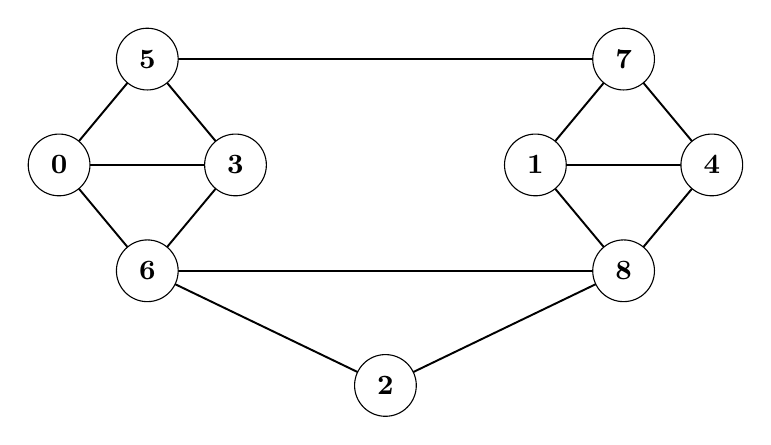
\begin{tikzpicture}[scale=1.12,every node/.style={transform shape}]
\Gcoords\Gedges\Gvertices
\end{tikzpicture}
\caption{\(G_9\): its nine labelled vertices and exactly fourteen edges, with graph6 \texttt{HCQTaXi}. The diamond units have bridges \(5\)--\(7\) and \(6\)--\(8\); vertex \(2\) joins \(6\) and \(8\). Edge fidelity is mechanically checked by \texttt{figure\_check.py}.}\label{fig:g9}
\end{figure}
\section{Definitions and conventions}
A configuration is a vector \(c:V(G)\to\mathbb{N}_0\) of total mass \(|c|=\sum_v c(v)\). One pebbling move \(u\to v\) requires an edge \(uv\) and \(c(u)\ge2\), replaces \(c\) by \(c-2e_u+e_v\), and lowers the mass by one. A configuration is \emph{stackable} if a finite sequence (possibly empty) ends with precisely one occupied vertex; it is \emph{clearable} if such a sequence ends with mass exactly one. Clearability implies stackability. The parameters \(\operatorname{stack}(G)\), for connected graphs with at least two vertices, and \(\operatorname{clear}(G)\), for connected non-bipartite graphs, are the least \(t\ge2\) for which \emph{every configuration of size exactly \(t\)} wins \cite{CSApril}.
A configuration is \emph{almost stacked} (AS) when some root \(r\) satisfies \(c(v)\le1\) for every \(v\ne r\). For each game \(P\in\{\mathrm{stack},\mathrm{clear}\}\) denote the losing configurations of mass \(t\) by \(\mathcal{L}_t^P\). Set
\begin{align*}
L_{\mathrm{all}}^P&=\max\{t\ge2:\mathcal{L}_t^P\ne\varnothing\},\\
L_{\mathrm{AS}}^P&=\max\{t\ge2:\mathcal{L}_t^P\text{ contains an AS input}\}.
\end{align*}
The critical form ASH$^*$ says the universal threshold equals the least \(t_0\ge2\) for which \emph{every almost stacked configuration of every size \(s\ge t_0\)} wins. Equivalently \(L_{\mathrm{all}}^P=L_{\mathrm{AS}}^P\) in the graph classes above. This is not the stronger printed \emph{least exact \(t\)} statement.
\begin{figure}[H]\centering
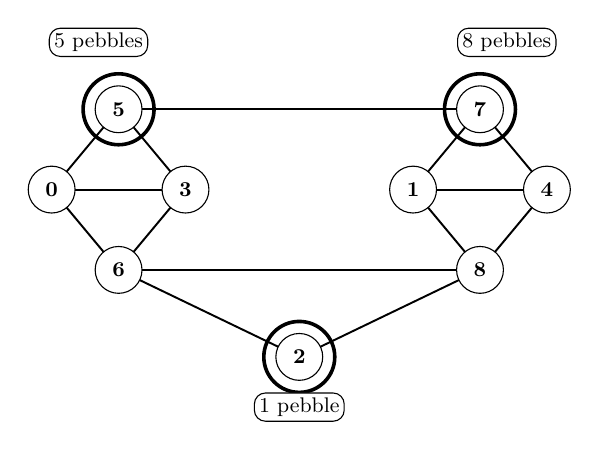
\begin{tikzpicture}[scale=.85,every node/.style={transform shape}]
\Gcoords\Gedges\Gvertices
\foreach \i in {2,5,7}{\draw[line width=1.3pt] (v\i) circle (5.3mm);}
\node[draw,fill=white,rounded corners,inner sep=2pt,font=\small] at ($(v5)+(-.3,1)$) {5 pebbles};
\node[draw,fill=white,rounded corners,inner sep=2pt,font=\small] at ($(v7)+(.4,1)$) {8 pebbles};
\node[draw,fill=white,rounded corners,inner sep=2pt,font=\small] at ($(v2)+(0,-.75)$) {1 pebble};
\end{tikzpicture}
\caption{The critical loser \(c^*\) has \(1+5+8=14\) pebbles, on vertices \(2,5,7\). Double-rimmed vertices are occupied; all others have zero. It is not AS, since \(5\) and \(7\) both have multiple pebbles. The automorphism \((0\,1)(3\,4)(5\,7)(6\,8)\) yields the other loser.}\label{fig:loser}
\end{figure}
\section{The printed pointwise formulation}
For a goal $P\in\{\mathrm{stack},\mathrm{clear}\}$ on a graph in the
applicable class, the printed hypothesis equates the universal threshold
with the least exact mass $t\ge2$ at which every almost-stacked
configuration succeeds. The following small examples disprove this
literal statement, without yet addressing the critical form.

\begin{proposition}[Pointwise counterexamples]\label{prop:pointwise}
Let $P_4$ be the path with edges $01,12,23$ and let $B$ be
the bull graph with edges $04,13,23,24,34$.
Every almost-stacked configuration of mass $12$ is stackable on
$P_4$, yet $(1,0,2,9)$ is not stackable.
Every almost-stacked configuration of mass $12$ is clearable on
$B$, yet $(1,9,0,2,0)$ is not clearable.
Both universal thresholds are $15$.
\end{proposition}

\begin{proof}
For either goal $P$ let $W_P(c)$ mean that $c$ wins. It satisfies
the terminating recursion
\[
 W_P(c)\Longleftrightarrow \mathrm{Goal}_P(c)\ \lor\
 \bigvee_{\substack{uv\in E(G)\\c(u)\ge2}}W_P(c-2e_u+e_v),
\]
since each move reduces mass. Enumeration of all weak compositions
of $12$ into four or five parts yields
\[
\begin{array}{c|r|r|r}
\text{graph/goal}&\text{AS inputs}&\text{AS winners}&
\text{all losers}\\ \hline
P_4/\mathrm{stack}&32&32&4\\
B/\mathrm{clear}&80&80&4
\end{array}
\]
The forward-reachable sets of the two stated losing vectors are closed
under legal moves, contain no goal, and have respectively $50$ and
$96$ elements. Winning sequences for all $32$ and $80$
almost-stacked inputs were independently checked, together with
these losing closures, in the public research record \cite{Repo}.
The companion \texttt{verify\_pointwise.py} independently checks the
same exact predicate and also finds losing counts $4,2,2,0$
at masses $12,13,14,15$, respectively, for each example.
The least all-winning almost-stacked mass is therefore at most $12$,
whereas the unrestricted threshold is $15$.
\end{proof}

\section{The critical form: a nine-vertex counterexample}
For either game, mass one is winning, so \(\mathcal{L}_1^P=\varnothing\).
Write \(\mathrm{Goal}_P(c)\) for an already stacked configuration
for STACK, and a single pebble for CLEAR. Every move reduces mass
by one, so for \(t\ge2\),
\begin{equation}\label{eq:rec}
\begin{aligned}
c\in\mathcal{L}_t^P\quad\Longleftrightarrow\quad&
 |c|=t,\ \neg\mathrm{Goal}_P(c),\\
&\text{every legal successor of }c\text{ lies in }\mathcal{L}_{t-1}^P.
\end{aligned}
\end{equation}
The goal exclusion is essential for STACK: a single pile is already
a winning goal even when all its legal successors are losing.
This is a precise equivalence, including no-move losses. Every loser is a 0--1 vector or is obtained by reversing a move from the previous losing layer. Therefore the complete candidate set can be chosen as
\begin{equation}\label{eq:candidate}
\begin{aligned}
\mathcal C_t^P={}&\{c\in\{0,1\}^{V}:|c|=t\}\\
&{}\cup\{s+2e_u-e_v:s\in\mathcal L_{t-1}^P,\ uv\in E,\ s(v)\ge1\}.
\end{aligned}
\end{equation}
Formula \eqref{eq:rec} retains exactly the losing members of \eqref{eq:candidate}. For an arbitrary losing \(c\) with a move \(u\to v\), its successor is necessarily losing by \eqref{eq:rec}, and reversing the move recovers \(c\). If there is no move then every coordinate is at most one on a graph without isolated vertices. Thus candidate completeness and soundness do not assume the result.
\begin{proposition}[Certified finite ingredients]\label{prop:cert}
In each of STACK and CLEAR on \(G_9\):
\(\mathcal L_{14}=\{c^*,c^{*\prime}\}\), \(\mathcal L_{15}=\varnothing\),
each layer \(2\le t\le14\) is nonempty, and
\(w=(0,0,1,0,1,11,0,0,0)\) is an AS loser of mass \(13\).
\end{proposition}
\begin{proof}[Computer-assisted, Lean kernel-checked]
The Lean development defines the legal-move reflexive-transitive reachability predicate and the separate STACK and CLEAR goals in \path{formal/AlmostStacked/Defs.lean}. Its \texttt{Checker.lean} proves that an encoded ordered losing-layer tree matches the mathematical losing predicate using the successor equation, ordered-tree membership, goal exclusion and a formally proved candidate-completeness condition. The data arrays are untrusted generated candidates. Each Boolean finite-layer condition is evaluated inside the Lean kernel with \texttt{decide +kernel}; the chain of layers \(2,\ldots,15\) is checked separately for STACK and CLEAR. The exact size-\(14\) characterisation, size-\(15\) emptiness, \(w\), and all lower-layer witnesses are proved in \path{formal/AlmostStacked/Main.lean}. No claim of hand enumeration is made.
\end{proof}
\begin{table}[H]\centering\small
\begin{tabular}{r rr@{\quad}r rr}\toprule
Mass & STACK & CLEAR & Mass & STACK & CLEAR\\\midrule
2&36&36&9&2510&2510\\
3&128&137&10&1301&1301\\
4&383&384&11&473&473\\
5&930&932&12&124&124\\
6&1862&1863&13&21&21\\
7&2887&2887&14&2&2\\
8&3280&3280&15&0&0\\\bottomrule
\end{tabular}
\caption{Exact number of losing configurations at each mass; recorded as cold-rechecked finite layers. These are not estimates.}\label{tab:counts}
\end{table}
\begin{lemma}[Monotonicity above the order]\label{lem:monotonic}
If \(G\) has \(n\) vertices and no isolated vertices and all configurations of mass \(t\ge n\) win a given goal (STACK or CLEAR), then every configuration of every mass \(s\ge t\) wins.
\end{lemma}
\begin{proof}
If \(s>t\ge n\), the pigeonhole principle gives a vertex holding at least two pebbles. Move once along an incident edge; the resulting mass is \(s-1\). Descending induction finishes.
\end{proof}
\begin{proof}[Proof of Theorem~\ref{thm:main}]
The graph is connected by inspection of its listed edges, and has the odd triangle \(0,3,5\). The certificate proposition gives all-size-\(15\) success; Lemma~\ref{lem:monotonic} propagates it above \(15\). The nonempty layers \(2,\ldots,14\) establish the least guaranteed exact threshold \(15\). At mass \(14\), the two losers both have two occupied vertices with at least two pebbles. Thus no AS input loses at \(14\); every larger input wins; and the specified AS input \(w\) loses at \(13\). Hence \(L_{\rm AS}=13\), \(L_{\rm all}=14\) for both games. This refutes the two critical universal clauses.
\end{proof}
\section{Formal verification and scope}
The Lean development proves the relevant definitions and checker correctness, then uses kernel evaluation to certify the finite STACK and CLEAR losing layers on \(G_9\). The twenty-five formal targets, including both universal negations, are specified in \texttt{formal/Challenge.lean}. The result was registered in the Palomar Registry on 27 October 2026 as \PalomarEntry\ \cite{PalomarG9}; the registered record links the archived source and identifies its formal theorem names. This formal verification does not constitute a claim of uniqueness or priority.
An order-\(9\) witness does not prove uniqueness in the class of all order-\(9\) graphs, given outstanding independently unverified atlas cases. The suggested infinite bridge families remain conjectural. The earlier tree stacking theorem \cite{TreeStack} is independent prior work.
\section*{Availability, acknowledgements and declarations}
Source: \url{https://github.com/jfairfaxball-348/Almost-Stacked-Proof}. Frozen Lean submission snapshot: \texttt{palomar/submission} at commit \texttt{34363e522213}. The Palomar archive preserves the registered source commit \texttt{358729c65c19} (full commit identifiers are in \texttt{paper/README.md}). Palomar record: \PalomarEntry. To regenerate diagrams and check graph integrity run \texttt{python3 figure\_check.py}; build commands and environment are in \texttt{paper/README.md}. The pebbling parameters and motivating conjecture are due to Tam\'as Csern\'ak and Lajos Soukup \cite{CSApril,CSOctober}. AI was used substantially in the formalisation and manuscript creation. The named author remains responsible for the paper.
\bibliographystyle{plain}
\bibliography{references}
\end{document}
